\documentclass[11pt]{article}

\usepackage{float}
\usepackage{hyperref}
\usepackage{fullpage}
\usepackage{verbatim}
\usepackage{moreverb}
\usepackage{graphicx}
\usepackage{minted}
\let\verbatiminput=\verbatimtabinput
\def\verbatimtabsize{4\relax}

\begin{document}
\title{EECS 151/251A FPGA Lab\\
Lab 3: Useful Digital Circuits for Basic Signal Processing, Finite State Machines, Synchronous RAMS, and Synchronous Resets}

\author{Prof. Borivoje Nikolic \\
TA: Vighnesh Iyer \\Department of Electrical Engineering and Computer Sciences\\
College of Engineering, University of California, Berkeley}
\date{}
\maketitle

\section{Before You Start This Lab}

Before you proceed with the contents of this lab, we suggest that you look through three documents that will help you better understand some concepts we will be covering.

\begin{enumerate}
	\item \textbf{labs\_fa16/docs/Verilog/verilog\_fsm.pdf} - Goes over concepts of FSM in Verilog. Provides an example of  implementing FSM's in Verilog and pitfalls to watch out for.
	
	\item \url{http://www.labbookpages.co.uk/electronics/debounce.html} - Read "What is Switch Bounce" section to get idea of why we need a debouncer circuit. Read the "Digital Switch Debouncing" section to get a general overview of the circuit, its parts, and their purpose. You may want to pay attention to the purpose of the synchronizer as meta-stability is something you will go over in class. 
	
	\item \url{http://www.xilinx.com/products/boards/s3estarter/files/s3esk_rotary_encoder_interface.pdf} - Read page 5 (Rotary Encoder and Signals) to get an idea of how the encoder works and the signal it generates. You can read the next few pages to get a better idea of how to use the signals. 

\end{enumerate}

In the first couple sections of this lab, we will be revisiting the circuit you did in lab 2 and reconfirming functionality with actual music generated by the updated scripts. Then we will be going over some new circuits that you will be using in future assignments.

\subsection{Helpful Hint: Synthesis Warnings and Errors}
At various times in this lab, things will just not work on the FPGA or in simulation. To help with debugging, you can run \verb|make synth| in the \verb|lab2/| folder. This will just run \verb|xst| which will only take a few seconds. Then you should run \verb|make report|. In the window that opened, click on \verb|Synthesis Messages| on the left under \verb|Errors and Warnings|. Any synthesis warnings you see here are a possible alert to some issue in your circuit. If you don't understand a warning, ask a TA; it almost always reveals some issue in your RTL.

If your reports indicate there are no issues but you still have problems, please make sure that it is working in simulation. There is one case related to how memory is generated where you will likely get different results between simulation and actual FPGA behavior but we do not expect it to occur in this lab. This is an issue we will discuss in later in the lab. 

Also, you should try to keep the bit widths of the ROM and \verb|music_streamer| address consistently large enough. You can still keep the ROM data width 24 bits but for the address width you will want to make it at least 12 bits.  
\section{Lab Overview}

In this lab, we will begin by taking your \verb|tone_generator| and \verb|music_streamer| design from Lab 2 and feeding it parts of real music. We will learn about circuits to take the signals generated by our buttons and rotary encoder and convert them into a digital signal we can use within our digital clock domain. You will be using the LED's to confirm they are working correctly. We will also be going over properly using synchronous resets to refresh the state of the circuits. 

\section{Tone\_generator With Music}

\subsection{Overview of Your Tone\_generator and Music\_streamer}

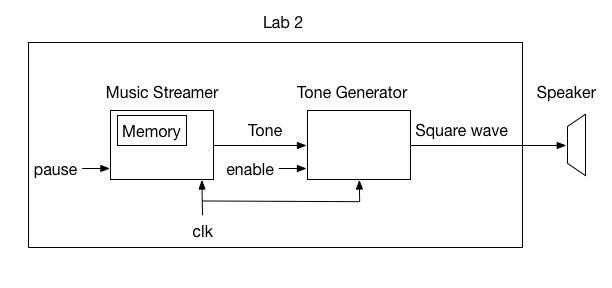
\includegraphics[width=\textwidth]{images/lab2_fig1.png}

We included this diagram so you can review the circuit you made in lab 2. There are two main modules that you created: \verb|tone_generator| and \verb|music_streamer|. 

Your \verb|tone_generator| should take an input signal representing the tone or frequency you want to play and output an oscillating signal that goes to the speaker. It has an enable signal that basically turns if off and on, and this enable signal should be hooked up to one of the DIP switches.  

Your \verb|music_streamer| is responsible for providing the input signal to your \verb|tone_generator| so it knows what frequency to play. Inside this generator is the memory (ROM for lab 2), that holds the frequencies you want to play. Your music generator will output one tone for a certain amount of time (1/5 of a second for lab 2) before updating its address to its memory. This new address should point to the next frequency you want to play. Your \verb|music_streamer| will keep incrementing its address until it reaches the end of the ROM in which case, it reset back to the first address, and plays your tones from the beginning again. 

We will be adding two new circuits to what we already have to give our music circuit more functionality.

\subsection{Playing Music}
Run \verb|git pull| in your git cloned \verb|labs_fa16| directory to fetch the latest skeleton files.

Begin by copying your \verb|tone_generator| and \verb|music_streamer| implementation into the \newline \verb|lab2/tone_generator.v| and \verb|lab2/music_streamer.v| files. Run 
\begin{minted}{verilog}
python musicXML_parser.py input_xml_file.xml output_text_file.txt
\end{minted}
This basically converts some sheet music (in the form of an XML file) into the text files you used in previous labs to generate the ROMs. We provided some XML files for you to use. Some of these should sound familiar. Additionally, if you want, you can go online and find XML files for other pieces you want to play. Now run the same command from the previous lab
\begin{minted}{verilog}
python rom_generator.py src/rom.v output_text_file.txt 4096 24
\end{minted}

Keep in mind there are a few new things you want to take into account. 

- We've made the depth of the ROM 4096 entries now but the it is likely the piece of music you will be playing is not that long. The remainder of memory is likely a bunch of empty zeroes. However, we want to loop our music without waiting a long pause in between each iteration.

The ROM module generated by the script should now have an extra output called \verb|last_address| which outputs the last address in memory that is actually part of the song. Your task is to use this \verb|last_address| in your \verb|music_streamer| module and reset at this address rather than 128 as with the previous lab.

- DO NOT forget to change the address width in your module; if the memory can now hold 4096 entries, how many bits should the address be? (it was mentioned previously in the lab)

- Another small change we made is how long we want each entry in the memory to play. Instead of 1/5 of a second, change your \verb|music_streamer| such that it now changes addresses every 1/25 of a second. We've made changes to the script when converting the music. Changing it to 1/25 second makes the music play more naturally.

Once you are done, recompile and program the FPGA. It should now be able to play one of the tunes we provided and loop without any silence in between.
\newline
* One issue you probably won't run into but should be aware of is that the tools will use distributed memory as long as our ROM module is small enough which is asynchronous. If the ROM we specify is too big, then it will be use block memory instead which is synchronous and your \verb|music_streamer| currently does not expect to use synchronous memory.

\section{Synchronizer, Debouncer, and Rotary Encoder}

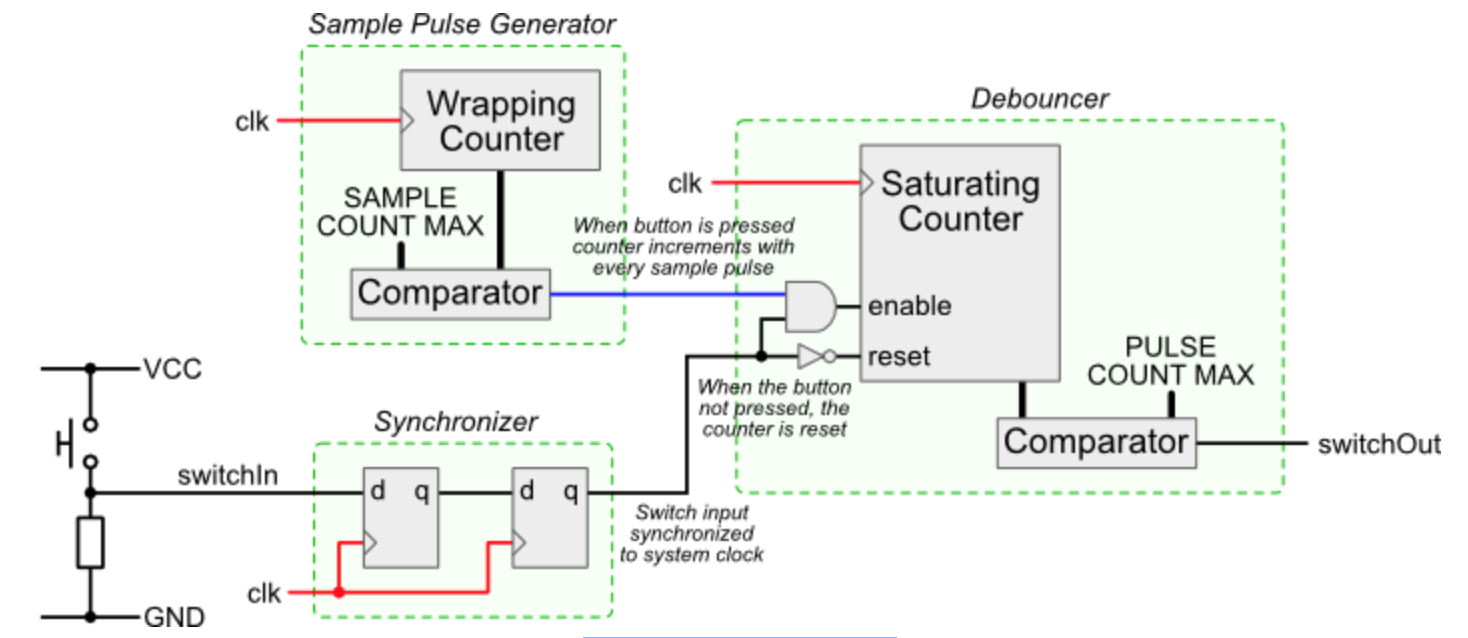
\includegraphics[width=\textwidth]{images/lab2_fig2.png}

Here is a overview of the debouncer circuit which includes the synchronizer circuit which you will also be using in the rotary encoder. 

\subsection{Synchronizer}
Generally, digital signals can be interpreted as 0's and 1's. However, in reality these correspond to low and high voltages and there are other states that can occur. The one we will be concern with for this lab is the metastable state.

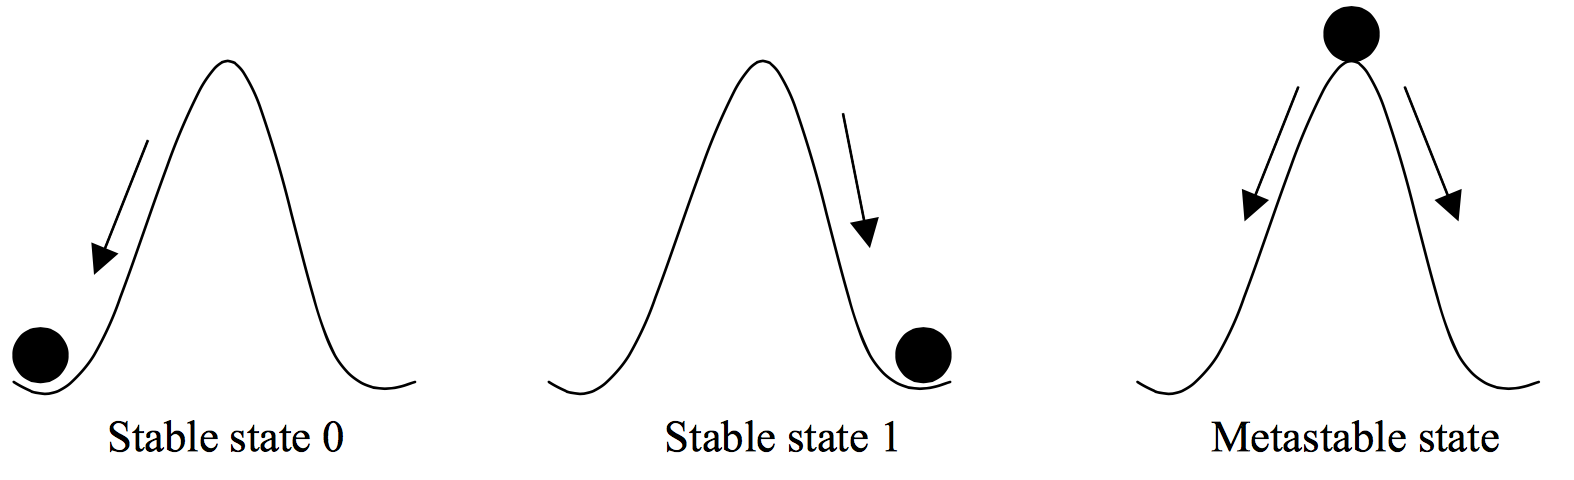
\includegraphics[width=\textwidth]{images/lab2_fig3.png}

Normally, when there are no clocking problems, we only have to worry about the high and low states. However, if there are timing issues, we can run into metastability  where a net is basically stuck between the two states. This is an oversimplification but what you ultimately need to know is that metastability is generally undesirable and we want a circuit to get rid of it. 

This synchronizer circuit we want you to implement for this lab is relatively simple. For one bit, its basically a pair a flip-flops. When a net is metastable it will eventually resolve to a high or low , although we want to avoid a metastable value from propagating to the rest of the circuit. Having a pair of flip-flops reduces the chance of the metastability propagating since this metastable state would have to last two clock cycles before moving on to the next part of the circuit.

\subsection{Debouncer}

For this lab, the debouncer circuit will basically take the signal from when you press a button on the FPGA and convert it into a digital signal. The reason we need a somewhat involved circuit for this is shown in the figure below.

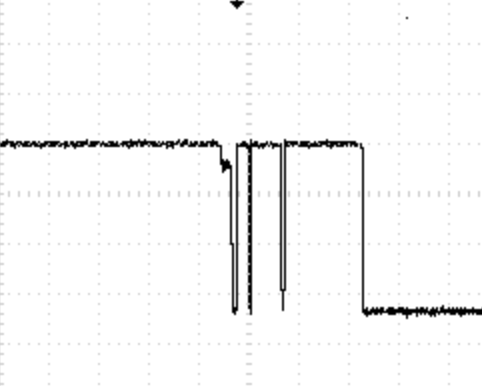
\includegraphics[width=\textwidth]{images/lab2_fig4.png}

When we press the button, we don't get a perfect stable signal. It "bounces" but we want a solid signal so we will use the circuit showed previously.

The one bit debouncer circuit we want you to implement consists of three main parts:

- the synchronizer which in our case will be outputting the digital signal of the buttons on our FPGA board being pressed

- the sample pulse generator which tells our main circuit to check the synchronizer output signal every n cycles by using a counter and telling the main circuit to sample every time the counter hits max and resets the counter

- the debouncer which works very similarly to the the sample pulse generator. Every time the sample pulse generator tells this debouncer to sample and our synchronizer output was high, that means the button was held for that sample. Once we reach a certain number of logical high sample values, we established that the button was pushed. You might get the impression the button has to be pressed relatively longer for all the circuitry to realize it has been pressed, but considering how fast the clock is, you normally pushing the button should be enough time if you didn't make the counter values unreasonable large.

We'll want you to make a debouncer circuit for 7 buttons: the 5 cross oriented buttons on the board, the reset button, and the rotary encoder also acts as a button.

\subsection{Rotary Encoder}

The rotary encoder consists of circuit that basically has two switches that go high as you rotate the wheel. 

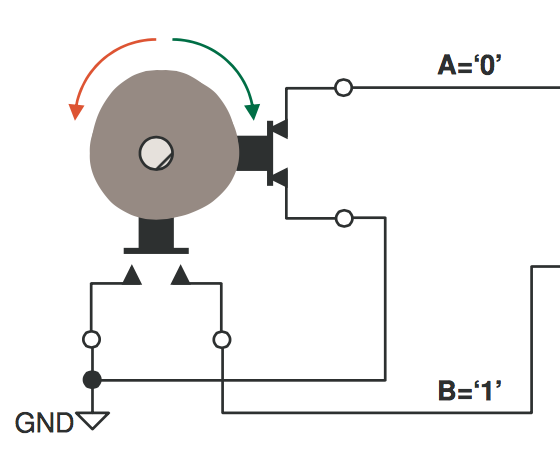
\includegraphics[width=\textwidth]{images/lab2_fig5.png}

Our main concern is finding out which direction the wheel turned. The following figure illustrates how we will do so. Basically, if the pulse from A happens before the pulse from B, it indicates that a the wheel has been a certain way and if the wheel is spun in the opposite direction then B's pulse will occur before A. We will take advantage of the fact that we will have two different rising edges to find the direction the wheel was turned.

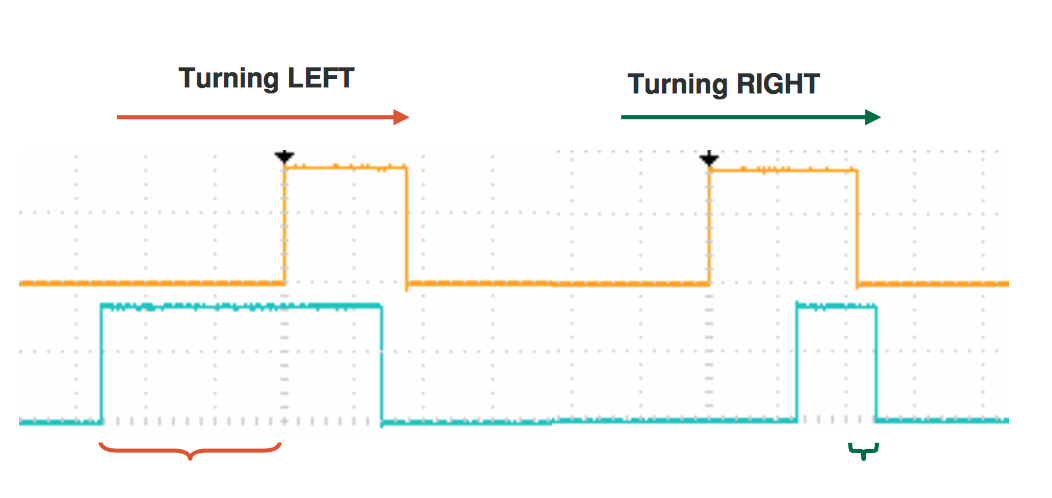
\includegraphics[width=\textwidth]{images/lab2_fig6.png}


\section{Conclusion}

\end{document}